\documentclass[12pt,letterpaper]{article}
\usepackage[utf8]{inputenc}
\usepackage[spanish]{babel}
\usepackage{graphicx}
\usepackage[left=2cm,right=2cm,top=2cm,bottom=2cm]{geometry}
\usepackage{graphicx} % figuras
% \usepackage{subfigure} % subfiguras
\usepackage{float} % para usar [H]
\usepackage{amsmath}
%\usepackage{txfonts}
\usepackage{stackrel} 
\usepackage{multirow}
\usepackage{enumerate} % enumerados
\renewcommand{\labelitemi}{$-$}
\renewcommand{\labelitemii}{$\cdot$}
% \author{}
% \title{Caratula}
\begin{document}

% Fancy Header and Footer
% \usepackage{fancyhdr}
% \pagestyle{fancy}
% \cfoot{}
% \rfoot{\thepage}
%

% \usepackage[hidelinks]{hyperref} % CREA HYPERVINCULOS EN INDICE

% \author{}
\title{Caratula}

\begin{titlepage}
\begin{center}
\large{UNIVERSIDAD PRIVADA DE TACNA}\\
\vspace*{-0.025in}
\begin{figure}[htb]
\begin{center}

\includegraphics[width=8cm]{./images/logo}
\end{center}
\end{figure}
\vspace*{0.15in}
INGENIERIA DE SISTEMAS  \\

\vspace*{0.5in}
\begin{large}
TITULO:\\
\end{large}

\vspace*{0.1in}
\begin{Large}
\textbf{INFORME DE PROYECTO} \\
\textbf{“GUIA DE INSTALACION DE GESTOR DE BASE DE DATOS DE ORACLE Y DE LA IMPLEMENTACION Y CONFIGURACION DE UNA BASE DE DATOS”} \\
\end{Large}

\vspace*{0.3in}
\begin{Large}
\textbf{CURSO:} \\
\end{Large}

\vspace*{0.1in}
\begin{large}
BASE DE DATOS II\\
\end{large}

\vspace*{0.3in}
\begin{Large}
\textbf{DOCENTE(ING):} \\
\end{Large}

\vspace*{0.1in}
\begin{large}
 Patrick Cuadros Quiroga\\
\end{large}

\vspace*{0.2in}
\vspace*{0.1in}
\begin{large}
Integrantes: \\
\begin{flushleft}
Moreno Mulluni Luis Angel		\hfill	(2017057864) \\
Layme Valeriano Diego 		\hfill	(2017057865) \\
Mamani Calisaya Yonathan 	           	\hfill	(2017057863) \\
\end{flushleft}
\end{large}
\end{center}

\end{titlepage}



\begin{center}
\textbf{COMO INSTALAR EL GESTOR DE BASE DE DATOS DE ORACLE EN WINDOWS SERVER 2012}
\end{center}

\begin{flushleft}
Instalar setup.exe del Sistema Gestion de Base de Datos Oracle 11g\\
Ejecutar instalador de SGBD Oracle 11g y aceptar instalación
\begin{center}
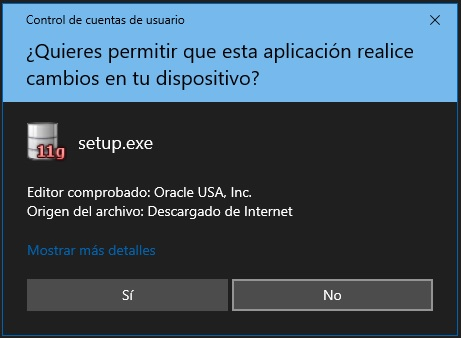
\includegraphics{images/image-01}\\
\end{center}
Nos aparecerá esta ventana en la cual esperaremos a que cargue la parte gráfica del instalador\\
\begin{center}
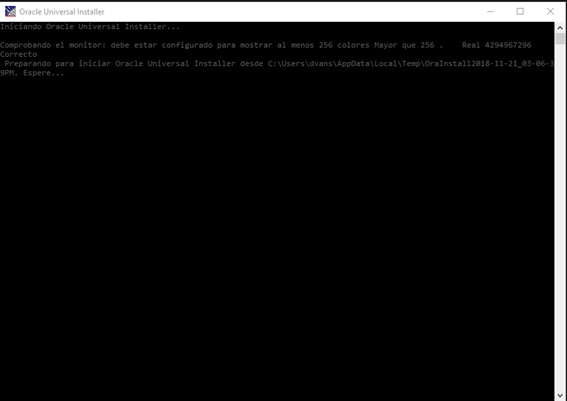
\includegraphics{images/image-02}\\
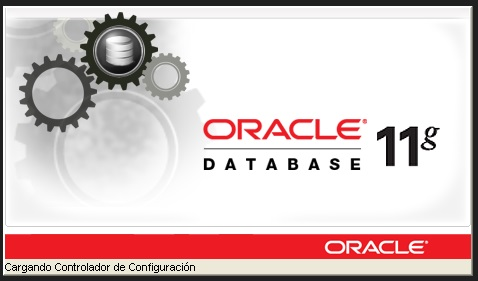
\includegraphics{images/image-03}\\
\end{center}
Nos saldrá una ventana en donde colocamos que si deseamos continua\\
\begin{center}
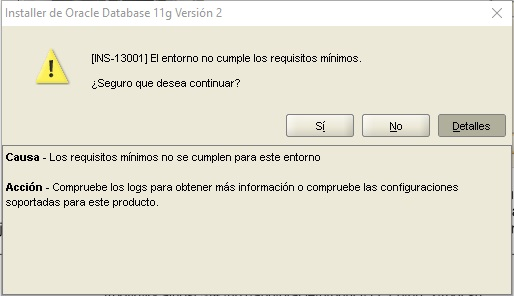
\includegraphics{images/image-04}\\
\end{center}
En esta parte presionamos en el boton siguiente\\
\begin{center}
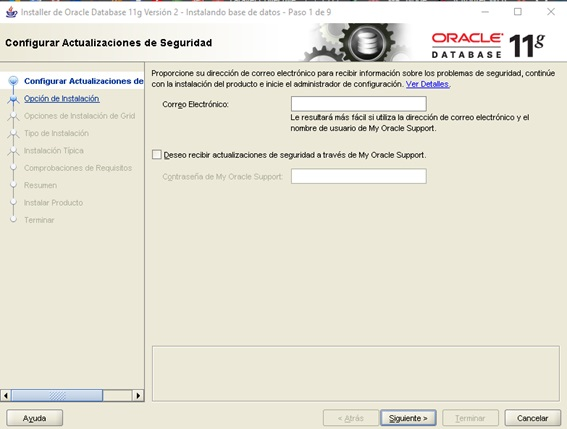
\includegraphics{images/image-05}\\
\end{center}
Nos saldrá esta ventana en el cual presionamos en el botón no porque no asignamos un correo\\
\begin{center}
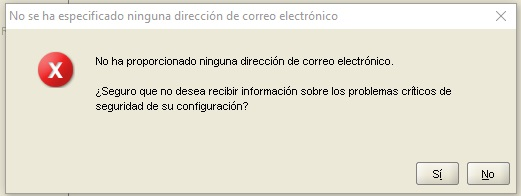
\includegraphics{images/image-06}\\
\end{center}
Selecionamos la opcion Crear y configurar base de datos , luego presionamos el boton siguiente\\
\begin{center}
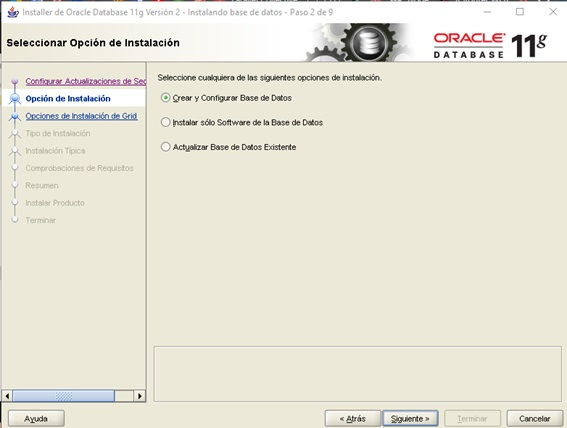
\includegraphics{images/image-07}\\
\end{center}
\end{flushleft}
\begin{flushleft}
Seleccionamos la opción Clase de Escritorio y luego en el botón siguiente\\
\begin{center}
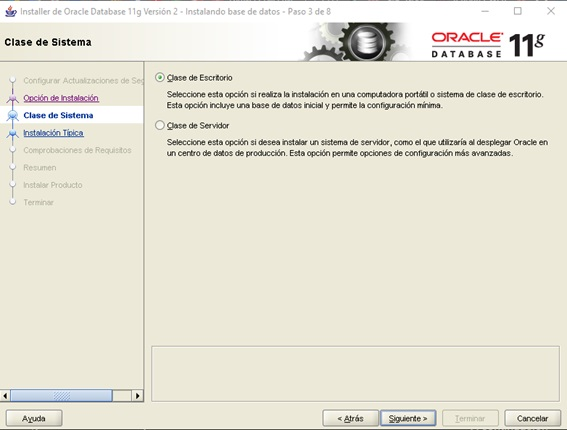
\includegraphics{images/image-08}\\
\end{center}
En esta parte de la instalación llenamos todo el formulario y luego en el botón siguiente\\
\begin{center}
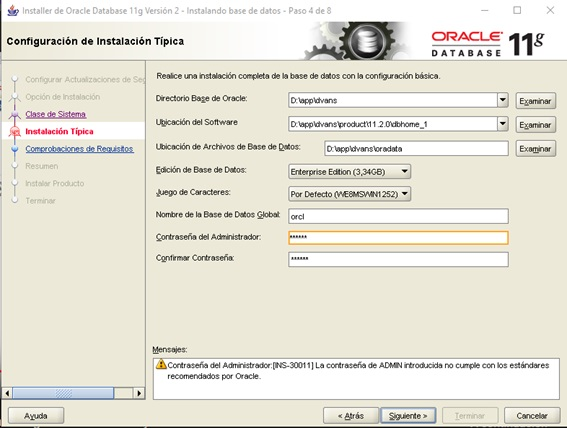
\includegraphics{images/image-09}\\
\end{center}
En caso de introducir una clave que no cumpla con los estándares nos saldrá esta ventana y colocamos en que si, para confirmar que estamos seguros de continuar.\\
\begin{center}
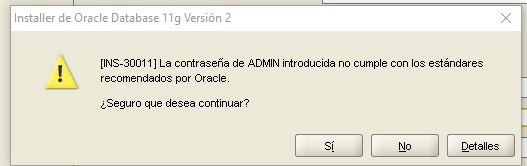
\includegraphics{images/image-10}\\
\end{center}
En esta ventana presionamos en el botón terminar\\
\begin{center}
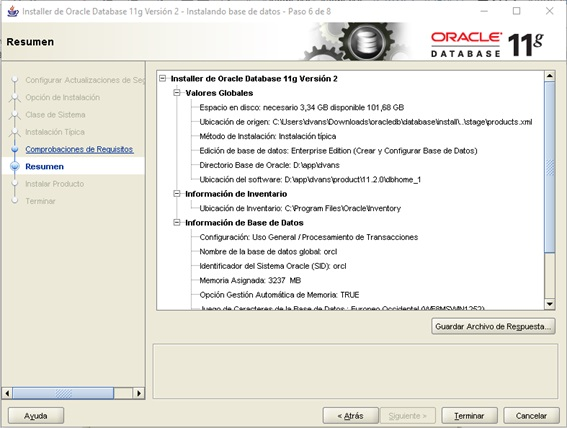
\includegraphics{images/image-11}\\
\end{center}
Luego empezara realizar la instalación\\
\begin{center}
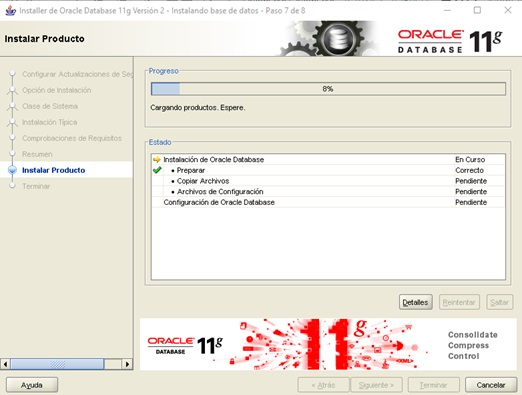
\includegraphics{images/image-12}\\
\end{center}
Adicionalmente aparecerá el asistente de configuración de bases de datos en el cual no debemos parar el proceso de configuración\\
\begin{center}
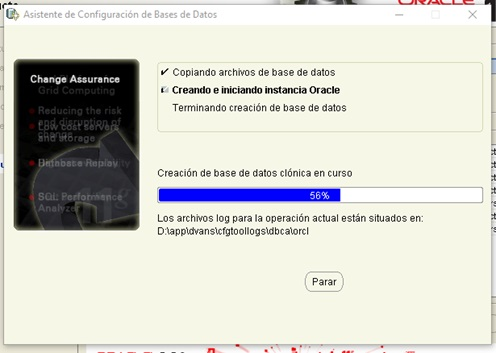
\includegraphics{images/image-13}\\
\end{center}
Una vez terminado la instalación el asistente nos mostrara esta ventana en la que debemos aceptar\\
\begin{center}
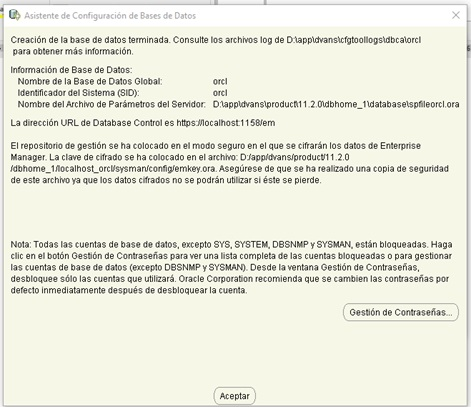
\includegraphics{images/image-14}\\
\end{center}
Finalmente se mostrará esta ventana indicándonos la URL donde se esta ejecutando el ENTERPRISE MANAGE DATABASE CONTROL y para finalizar presionamos el botón cerrar\\
\begin{center}
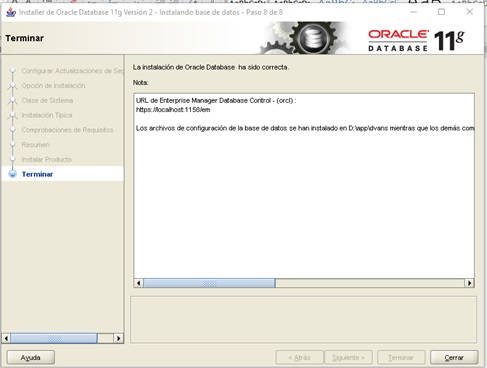
\includegraphics{images/image-15}\\
\end{center}
Abrimos la URL de ENTERPRISE MANAGE DATABASE CONTROL, de modo que comprobamos que la instalación se realizó correctamente. En esta ventana nos pedirá usuario y contraseña, por defecto colocamos “sys” como usuario y “oracle” como como contraseña, luego conectamos presionando en el botón conectar\\
\begin{center}
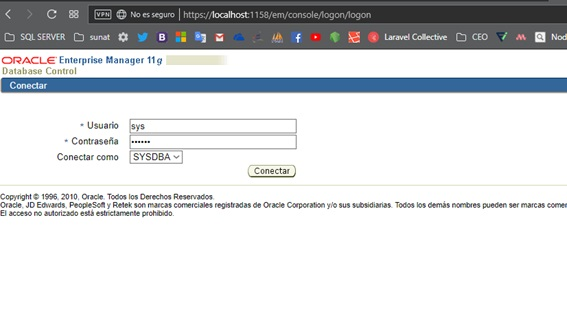
\includegraphics{images/image-16}\\
\end{center}
Una vez logueados correctamente nos aparecerá esta página\\
\begin{center}
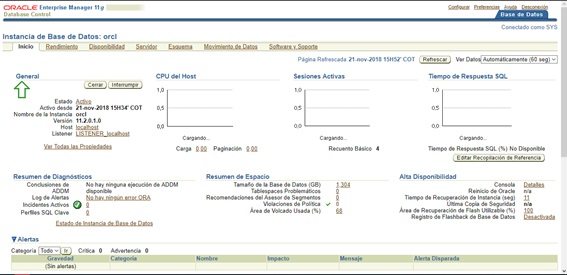
\includegraphics{images/image-17}\\
\end{center}
\end{flushleft}
\begin{flushleft}
Iniciamos una nueva conexión con el SQL DEVELOPER, aquí colocaremos, nombre de la conexión, el usuario sys, contraseña: Oracle, Tipo de conexión Básico, Rol: SYSDBA, Nombre del host: localhost, puerto 1521, SID: orcl\\
\begin{center}
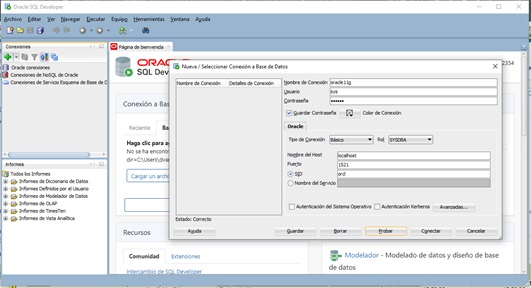
\includegraphics{images/image-18}\\
\end{center}
Una vez conectados creamos el usuario DBA1 y le otorgamos permisos con el comando GRANT\\
\begin{center}
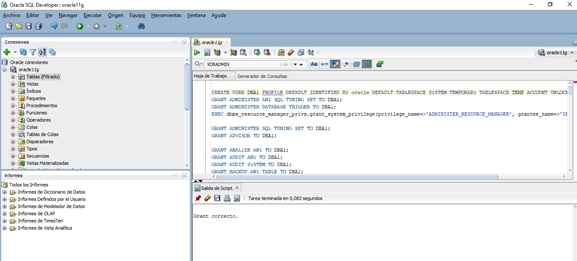
\includegraphics{images/image-19}\\
\end{center}
En este paso regresamos a la URL del ENTERPRISE MANAGE DATABASE CONTROL y nos dirigimos a link Configurar situado en la parte derecha superior de la ventana\\
\begin{center}
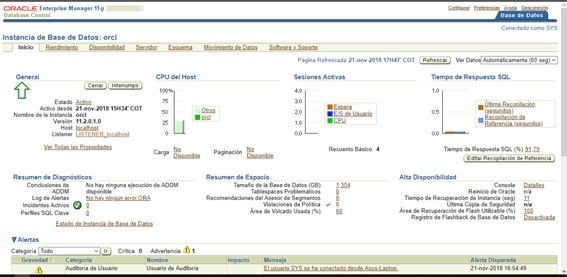
\includegraphics{images/image-20}\\
\end{center}
Después de hacer Clic nos mostrara la página de configuración, en donde damos clic en el link Administradores del menú situado al lado izquierdo de la ventana\\
\begin{center}
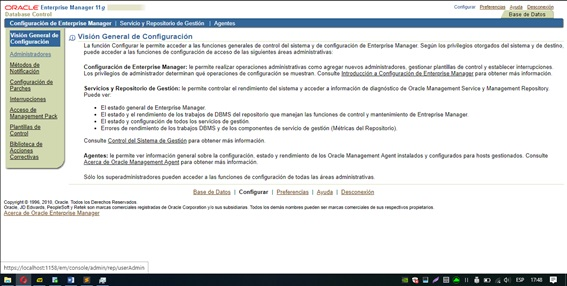
\includegraphics{images/image-21}\\
\end{center}
Después nos cargara esta página donde presionamos en el botón crear\\
\begin{center}
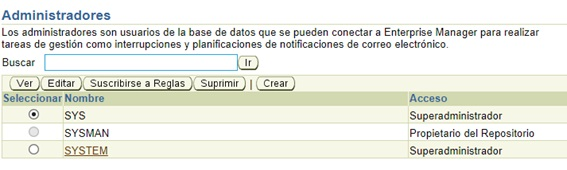
\includegraphics{images/image-22}\\
\end{center}
En esta página seleccionaremos el usuario previamente creado, asignaremos una dirección de correo electrónico y cambiamos el privilegio de administrador a SUPERADMINISTRADOR\\
\begin{center}
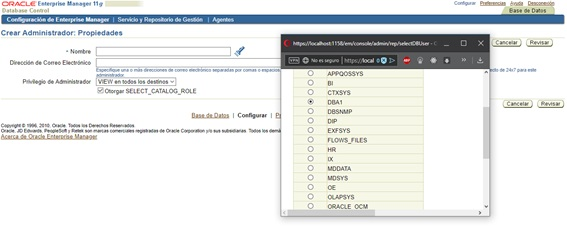
\includegraphics{images/image-23}\\
\end{center}
En esta página seleccionaremos al usuario DBA1 y luego presionamos en el botón seleccionar\\
\begin{center}
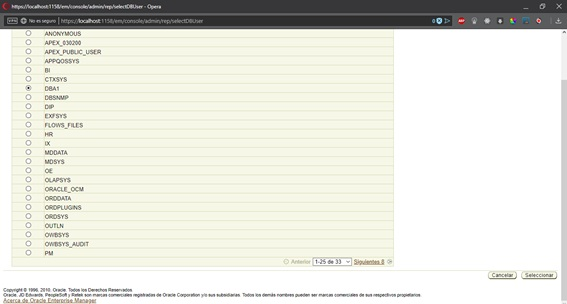
\includegraphics{images/image-24}\\
\end{center}
Una vez llenado el formulario para crear al USUARIO DBA1, presionamos en el botón revisar\\
\begin{center}
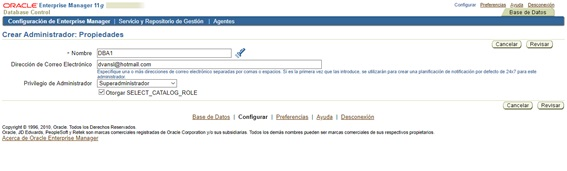
\includegraphics{images/image-25}\\
\end{center}
Luego nos saldrá otra página para confirmar la creación, para ello presionamos en el botón Terminar\\
\begin{center}
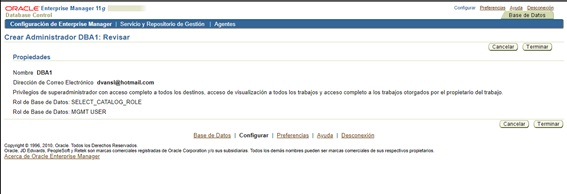
\includegraphics{images/image-26}\\
\end{center}
Luego verificamos en la página de Administrador, en donde debe figurar nuestro usuario debidamente creado\\
\begin{center}
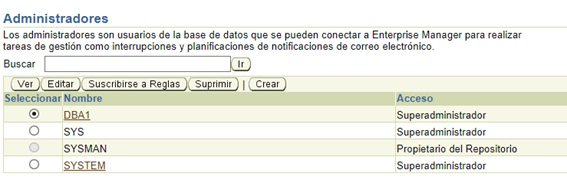
\includegraphics{images/image-27}\\
\end{center}
En este paso crearemos un tablespace para nuestro proyecto, para ellos nos dirigimos a la pestaña Servidor y luego al link Tablespaces\\
\begin{center}
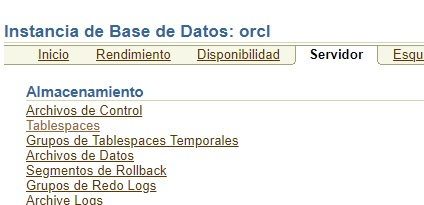
\includegraphics{images/image-28}\\
\end{center}
Luego nos mostrara la página para crear un tablespace\\
\begin{center}
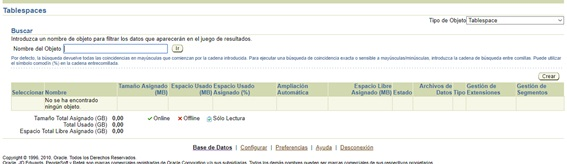
\includegraphics{images/image-29}\\
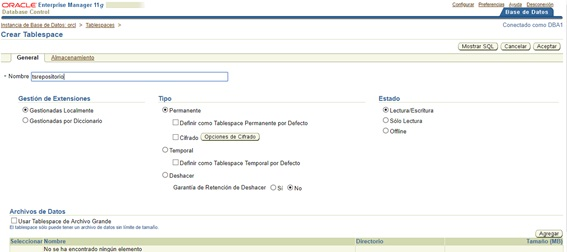
\includegraphics{images/image-30}\\
\end{center}
En esta ventana crearemos una tabla de espacio para nuestra base de datos, para ellos llenaremos todos los campos necesarios del formulario y luego presionamos en el botón continuar\\
\begin{center}
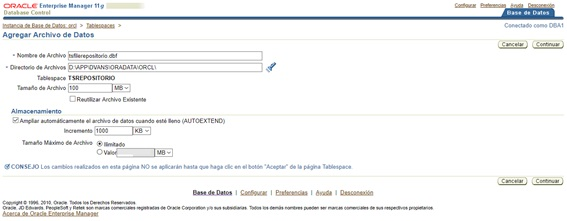
\includegraphics{images/image-31}\\
\end{center}
Luego en esta ventana colocaremos el nombre de la tabla de espacio y presionaremos en el botón aceptar\\
\begin{center}
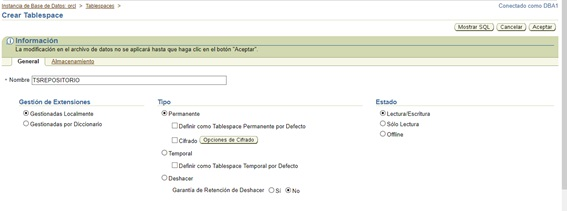
\includegraphics{images/image-32}\\
\end{center}
Finalmente en esta parte verificamos que nuestra tabla de espacio este en la lista de tabla de espacio\\
\begin{center}
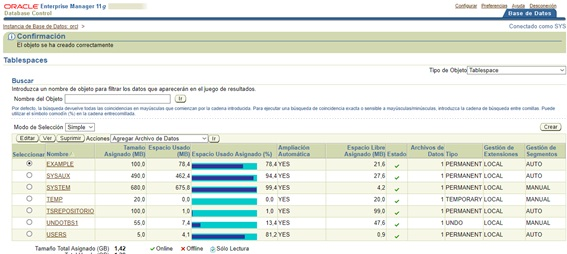
\includegraphics{images/image-33}\\
\end{center}
Finalmente crear las tablas de nuestra base de datos y las relacionaremos con el esquema DBA1\\
\begin{center}
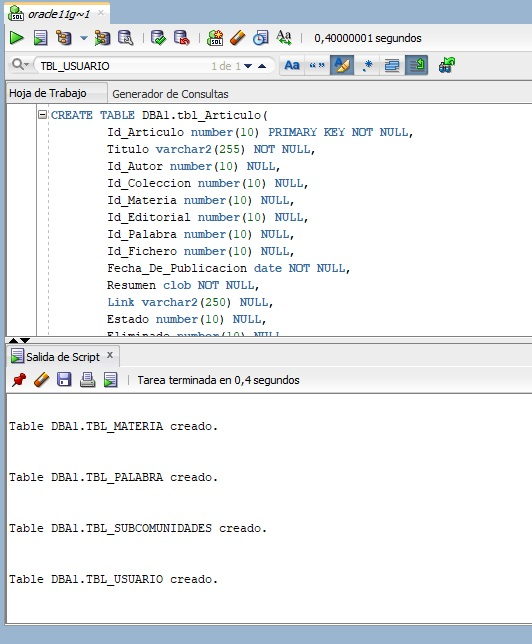
\includegraphics{images/image-34}\\
\end{center}
\end{flushleft}

\end{document}